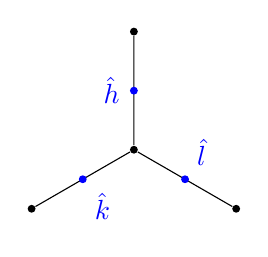
\begin{tikzpicture}
    [
  vertex/.style={
    circle,
    fill=black,
    minimum size=1mm,
    inner sep=0pt
  },
  hp/.style={
    circle,
    fill=blue,
    minimum size=1mm,
    inner sep=0pt
  },
  ->-/.style={
    decoration={
      markings,
      mark=at position 0.5 with {\arrow{#1}}
    },
    postaction={decorate}
  },
  scale=1.5
  ]
  \node (0) at (0,0) [vertex] {};
  \node (1) at (090:1) [vertex] {};
  \node (2) at (210:1) [vertex] {};
  \node (3) at (330:1) [vertex] {};
  \draw (0) -- (1)
  (0) -- (2)
  (0) -- (3);
  \node at (090:0.5) [hp,label={[blue]180:\(\mathfrak{\hat h}\)}] {};
  \node at (210:0.5) [hp,label={[blue]300:\(\mathfrak{\hat k}\)}] {};
  \node at (330:0.5) [hp,label={[blue]420:\(\mathfrak{\hat l}\)}] {};
\end{tikzpicture}
%%% Local Variables:
%%% mode: latex
%%% TeX-master: "../Master"
%%% End:
